\section{Grand Challenge Solution}
\label{sec:solution}

\begin{figure}[!ht]
	\centering
	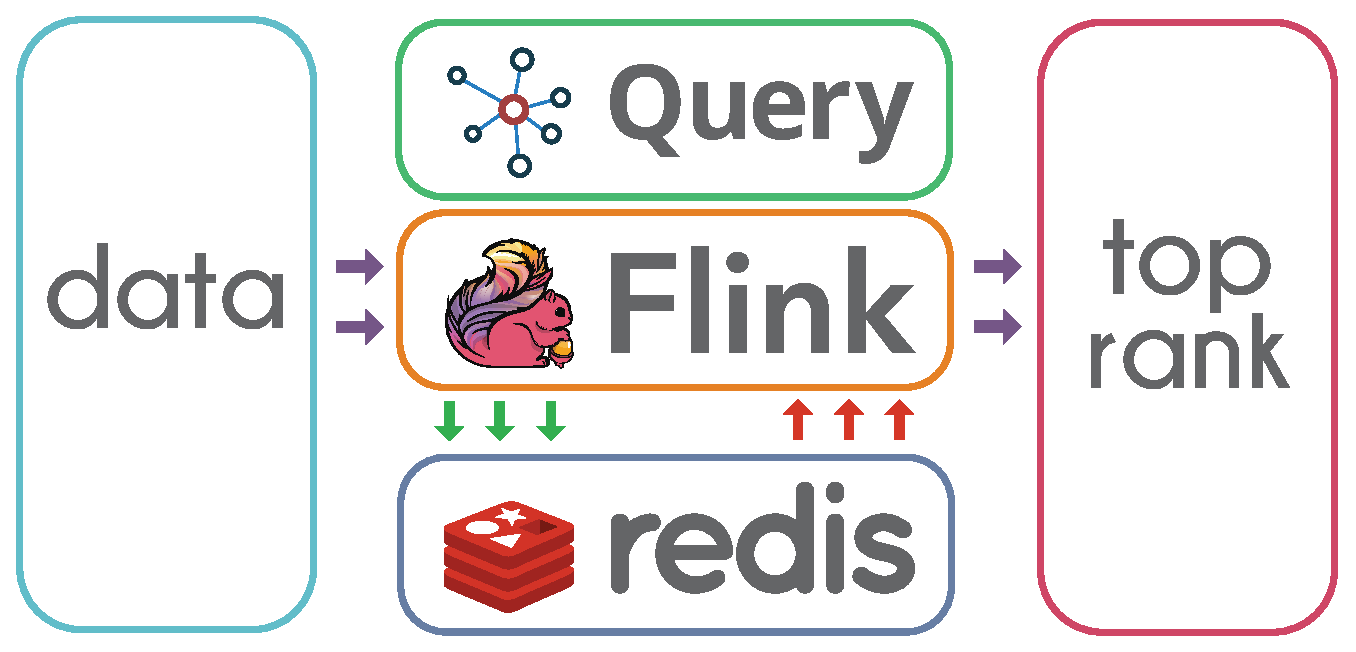
\includegraphics[width=0.35\textwidth]{fig/sostream-layered-architecture.eps}
%	\caption{The layered architecture.}
	\caption{High-level architecture of our solution.}
	\label{fig:sostream-layered-architecture}
\end{figure}

\begin{figure*}[!ht]
	\centering
	\includegraphics[width=.75\textwidth]{fig/query-1-architecture}
	\caption{The topology for Query 1.}
	\label{fig:q1-architecture}
\end{figure*}

The DEBS 2016 Grand Challenge poses two queries that require to efficiently handle several entities interacting each other (i.e., posts and comments) with the goal of discovering some complex dynamics which strongly depend on the passing of time. 
%
The design approach of our application revolves around two principles: parallelization and memory efficiency.
%
The application incorporates two independent solutions that answer the two queries.
%
Aside the specific details, both the solutions %can be easily described 
rely on a sequence of possibly parallel operators that apply stepwise transformations to the incoming events. 
%
Specifically, the application: (1) reads the events from the dataset stored on a file and pushes them within the system;  (2) computes the score associated to each relevant entity (i.e., post, comments); (3) on the basis of this score, determines the top-$k$ rankings with a two-step  approach (being $k$ a query-related parameter); 
and (4) emits the updated top-$k$ rankings. 
%
The meaning of score, and the way it is computed, changes according to the query.
For the first query, each post receives a score resulting from all its comments; the score provided by each comment and the score of the post itself slowly decay with the passing of time. 
%
For the second query, each comment receives a score depending on the size of the community that interacts with it within a given time window. 
%
Due to the great amount of data, computing the score represents the critical operation; therefore, we exploit parallelism to concurrently determine the score by working on independent partitions of the incoming events. 

To focus our effort on the application logic, we need a high-throughput and scalable stream processing framework.  
%
After having examined several alternatives, such as Storm\footnote{\url{http://storm.apache.org/}} and Spark\footnote{\url{http://spark.apache.org/}}, we have chosen Flink~\cite{Flink}, an open source project maintained by the Apache Software Foundation, because it shows promising performance with respect to other well-known frameworks.
%
Our application leverages some advanced features provided by Flink; the most relevant one is the feedback stream, i.e., a stream towards upstream operators, that we use to optimize the usage of memory by deleting expired posts which cannot compete for the top-$k$ ranking ones.
%
To answer the second query, the application also requires to efficiently store the social graph, which represents the users and their friendship relations, in order to periodically compute and retrieve the largest communities. 
%
We solve this problem through Redis~\cite{Redis},an in-memory data structure store, which avoids the bottleneck given by mass storage I/O. 
%
Figure~\ref{fig:sostream-layered-architecture} depicts a high-level overview of our solution.  
